\section{IR and Collinar Divergences}
Beyond the LO (Leading order) diagrams it happens singularities. To discuss about these consider first the process $ e^- e^+ \rightarrow q\bar{q}g $

\begin{figure}[ht!]
\centering
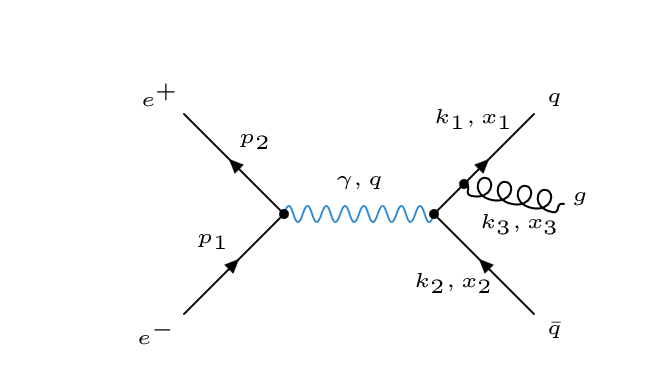
\includegraphics[width=0.85\textwidth]{images/Intro/IRCol.png}
\end{figure}

In order to calculate the cross section of this diagram, we have to consider the gluon emission from the antiquark. Since the calculation is quite long, we concentrate on the final result:
\begin{figure}[ht!]
\centering
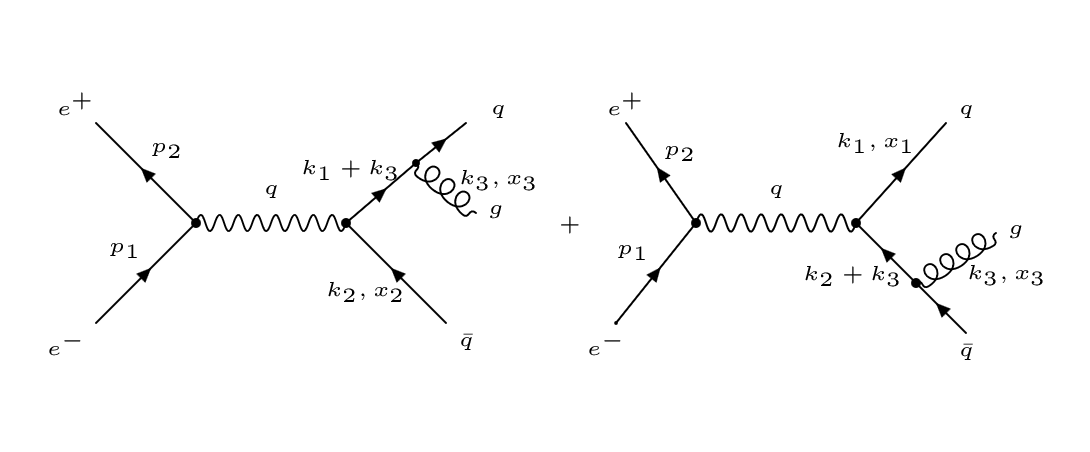
\includegraphics[width=0.85\textwidth]{images/Intro/IRColMatrix.png}
\caption{Left diagram $  e^- e^+ \rightarrow qg\bar{q} $ and right $ e^- e^+ \rightarrow q\bar{q}g $}
\end{figure}

\begin{equation}
\begin{split}
&A= \frac{\bar{u}(k_1)(-ig_s\gamma^{\nu}\times T^a)[-i(\not{k_1}+\not{k_3})](-iee_q \gamma^{\mu})v(k_2){\epsilon_{\mu}}^{\lambda_1}{\epsilon_{\nu}}^{\lambda_2*}}{(k_1 + k_3)^2}\\ 
&- \frac{\bar{u}(k_1)(-iee_q \gamma^{\mu})[i(\not{k_2}+\not{k_3})](-ig_s\gamma^{\nu}\times T^a)v(k_2){\epsilon_{\mu}}^{\lambda_1}{\epsilon_{\nu}}^{\lambda_2*}}{(k_1 + k_3)^2}\\
\Rightarrow &A=-g_s T^a[ \frac{\bar{u}\:\not{\epsilon}\:(\not{k_1}+\not{k_3})\:\Gamma \:v}{(k_1 + k_3)^2} - \frac{\bar{u}\:\Gamma\:(\not{k_2}+\not{k_3})\:\not{\epsilon} \:v}{(k_2 + k_3)^2}] \:\:\:\:\text{with} \:\:\Gamma=(-iee_q \gamma^{\mu}){\epsilon_{\mu}}^{\lambda_1}
\end{split}
\end{equation}
Under consideration that the partons are on-shell, we get:
\begin{equation}
 A=-g_s T^a[ \frac{\bar{u}\:\not{\epsilon}\:(\not{k_1}+\not{k_3})\:\Gamma \:v}{2k_1 \cdot k_3} - \frac{\bar{u}\:\Gamma\:(\not{k_2}+\not{k_3})\:\not{\epsilon} \:v}{2k_2 \cdot k_3}]
\end{equation}
In the soft limit with $k_0 \rightarrow 0$ we can factorize $ A_{soft} $ the amplitude in two parts:
\begin{equation}
 A=-g_s T^a[ \frac{k_1\:{\epsilon}}{k_1 \cdot k_3} - \frac{k_2\:{\epsilon}}{k_2 \cdot k_3}] A_{born} \:\:\:\:\:\:\:\:\:\:\:\:\:\:\:\:\:\text{with}\:\: A_{born}= \bar{u}\: \Gamma \:v
\end{equation}
 Which one contains all information about colour and momenta and $ A_{born} $ with all spin information.
If one calculates the cross section for it, one gets:
\begin{equation}
\begin{split}
A=&C_F g_s^2 \sigma^{born} \int \frac{d^3 k}{2k_0 (2{\pi})^3} 2(\frac{k_1 \cdot k_2}{(k_1 \cdot k_3)(k_2 \cdot k_3)})\\ 
&C_F g_s^2 \sigma^{born} \int dcos\: \theta\: \frac{d k_0}{k_0} \frac{4}{(1-cos\: \theta)(1+cos\: \theta)}
\end{split}
\end{equation}
We define the energy fraction by:
\begin{equation}
x_i = \frac{2E_i}{\sqrt{s}}=\frac{2q\: \cdot\: k_i}{s}
\end{equation}
One can show that $ \sum x_i =2  $ and thus, that only two of the $ xi $ are independent.

The final result is:
\begin{equation}
\frac{d^2 \sigma}{dx_1 dx_2}= (\frac{4\pi \alpha}{s})\sum {e_i}^2 
\frac{2\alpha_s}{3\pi} \frac{{x_1}^2+{x_2}^2}{(1-x_1)(1-x_2)}
\end{equation}

There are three singularities in regard with the final result. 
If the emitted photon is collinear to the outgoing quark or anti-quark $ (x_1 \rightarrow 1 \:\text{or}\: x_2 \rightarrow 1) $ and When the emitted gluon is very soft $ (x_1 \rightarrow 1\: \text{and}\: x_2 \rightarrow 1 )$.
The singularities come from the quark propagator in each diagram. The denominators contain according Feynmann rules terms with $\sim \frac{1}{(k_i + k_j)^2}  $. We can eliminate the quark mass under on-shell condition so that:
\begin{equation}
\frac{1}{(k_i + k_j)^2}=\frac{1}{2k_i \cdot k_j}=\frac{1}{2E_iE_j(1-cos\theta_{ij})}=\frac{1}{s(1- x_k)}
\end{equation} 
One can show all possibilities for three partons through a triangle:
\pagebreak

\begin{figure}[ht!]
\centering
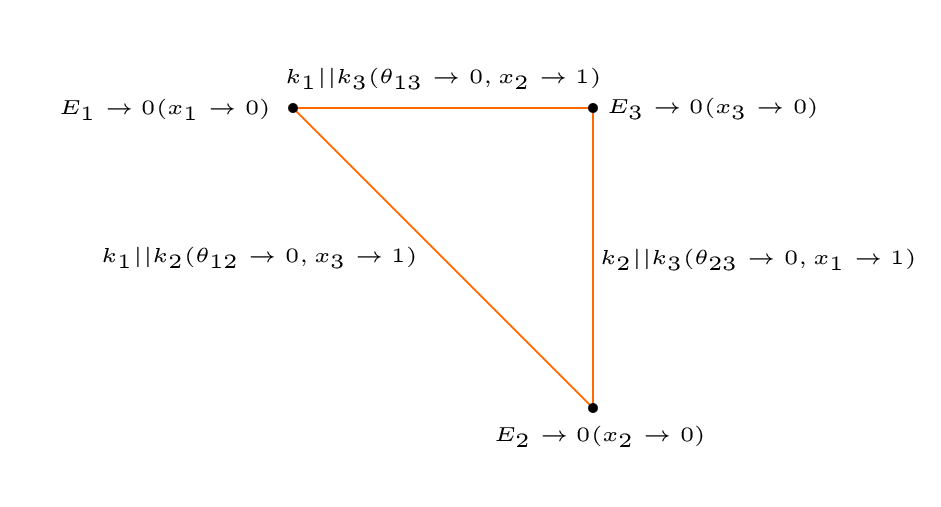
\includegraphics[width=0.85\textwidth]{images/Intro/triangle.png}
\end{figure}

fortunately, According to KLN-Theorem, IR singularities must cancel when summing the transition
rate over all degenerate (initial and nal) states
The sum of the integrals $ int_R $ and $ int_V $ above is finite. However, this is not true for the
individual contributions. The real part contains divergences due to soft and collinear
radiation of massless particles. While $ M_real $ itself is a tree level amplitude and thus
finite, the divergences show up upon integration over the phase space $ \int d \phi_3 $. In
R
V , the
phase space is the same as for the Born amplitude, but the loop integrals contained in
$ M_virt $ contain IR singularities.
\begin{figure}[ht!]
\centering
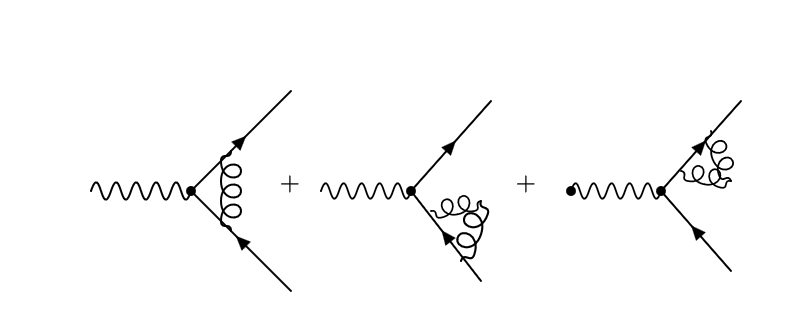
\includegraphics[width=0.85\textwidth]{images/Intro/virtual.png}
\end{figure}
We will use deep inelastic scattering (DIS) to show how the infrared singularities are absorbed in the parton distributions.

\section{Subtraction method}
\begin{equation}
|A|^2 = |{A^{(0)}}_m|^2 +  |{A^{(0)}}_{m+1}|^2+ 2Re({A^{(0)*}}_{n}{A^{(1)}}_{m})
\end{equation}
Whereby, $ |{A^{(0)}}_m|^2 $ is the tree level contribution (Born sector) from Lo and has no divergences, $ |{A^{(0)}}_{m+1}|^2+ 2Re({A^{(0)*}}_{m}{A^{(1)}}_{m}) $ comes from the NLO and they are separately divergent. The problem in this case is that Integrations cannot be combined due to different phase space dimensions:

\begin{equation}
\sigma^{NLO} = \int_{m+1} \partial \sigma^R +\int_{m} \partial \sigma^V
\end{equation}
The real and virtual contributions are both IR divergent and need to regularize in $ d = 4-2\epsilon $ dim.
To tackle this problem one can use the subtraction method in that way one add and subtract a local counter term $ \partial \sigma^A $ with same singularity structure as terms $ \partial \sigma^R $ to the integral. $ \partial \sigma^A $ approximates soft and collinear singularities of $ \partial \sigma^R  $.
\begin{equation}
\sigma^{NLO} = \int_{m+1} [\partial \sigma^R -\partial \sigma^A]+\int_{m} [\partial \sigma^V+\int_1 \partial \sigma^A]
\end{equation}
In this case, we can safely set $ \epsilon \rightarrow 0 $ for $ \partial \sigma^R |_{\epsilon \rightarrow 0}  -\partial \sigma^A |_{\epsilon \rightarrow 0} $ and run the integral numerically in 4-dim. On the other side, integrate over one-parton PS analytically
explicitly cancel poles and then set $ \epsilon \rightarrow 0 $.
\begin{equation}
\sigma^{NLO} = \int_{m+1} [\partial \sigma^R |_{\epsilon \rightarrow 0}  -\partial \sigma^A |_{\epsilon \rightarrow 0}]+\int_{m} [\partial \sigma^V+\int_1 \partial \sigma^A]_{\epsilon \rightarrow 0}
\end{equation}
The virtual contribution must be UV-finite:
\begin{equation}
\int_{m} partial \sigma^V= \int_m [\int_{loop} \partial {\sigma^V}_{bare} + {\sigma^V}_{Counter\:term}]
\end{equation}
The addition of $\int_1 \partial \sigma^A$ to the $ \int_{m} \partial \sigma^V $ ensures that IR poles are cancelled.
The bare and counter contribution are separately divergent and have also different integral dimensions. One can use the same idea with the subtraction method to solve this problem:
\begin{equation}
\int_{m} \partial \sigma^V +\int_{loop} \partial {\sigma^L}-\int_{loop} \partial {\sigma^L}= \int_m \int_{loop}[ \partial {\sigma^V}_{bare}- \partial {\sigma^L}] + \int_m[{\sigma^V}_{Counter\:term}+ \int_{loop} \partial {\sigma^L}]
\end{equation}


\begin{equation}
\sigma^{NLO} = \int_{m+1} [\partial \sigma^R -\partial \sigma^A]+ \int_m \int_{loop}[ \partial {\sigma^V}_{bare}- \partial {\sigma^L}] + \int_m[{\sigma^V}_{Counter\:term}+ \int_{loop} \partial {\sigma^L}+\partial \sigma^A]
\end{equation}

\section*{Determination of emission kernels}

\newpage
\section{Factorisation}
The hadron hadron scattering can be written as:
\begin{equation}
\sigma = \sum_{ij} \int dx_1 dx_2 f_i(x_1, \mu^2)f_j(x_2, \mu^2) \sigma_{ij}(x_1, x_2, Q^2/\mu^2... )
\end{equation}
\begin{figure}[h!]
\centering
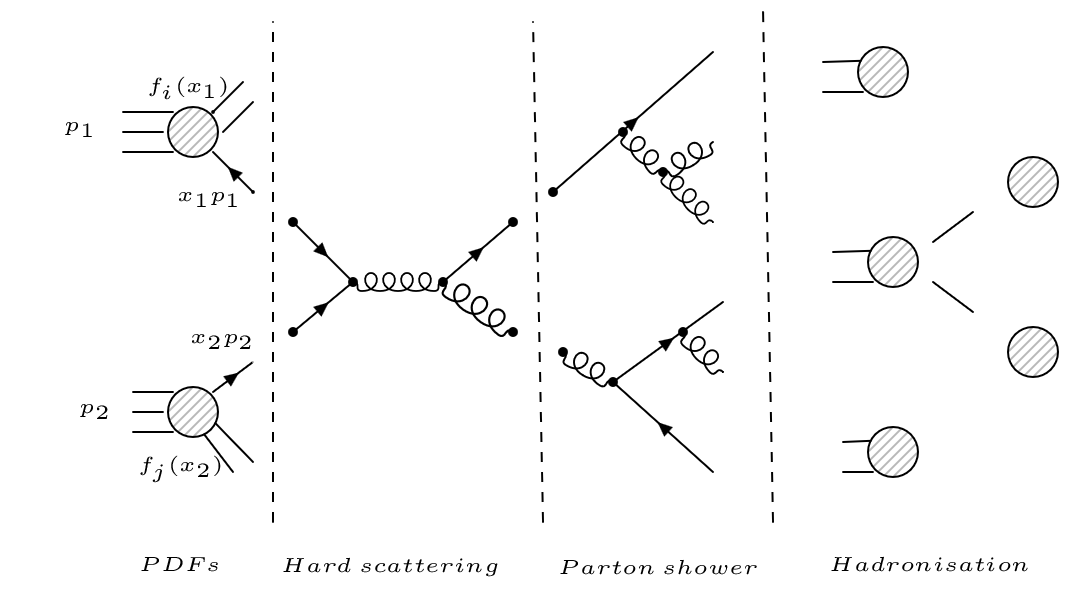
\includegraphics[width=0.85\textwidth]{images/Intro/Hard.png}
\end{figure}
Here the (arbitrary) factorisation scale $ \mu $ can be thought of
as the scale which separates the long and short-distance physics.
Roughly speaking, a parton with a transverse momentum less
than $ \mu $ is then considered to be part of the hadron structure and
is absorbed in the parton distribution. Partons with larger transverse
momenta participate in the hard scattering process with a
short-distance partonic cross-section.
The factorisation theorem also applies to deep inelastic scattering. The DIS cross section can be written as:
\begin{equation}
\frac{d^2 \sigma}{dx dQ^2}=\frac{4\pi \alpha^2}{x Q^4}[(1-y)F_2 (x, Q^2)+xy^2 F_1(x, Q^2)]
\end{equation}
In this case we need to introduce the structure function, is defined as the charge weighted sum of the parton momentum densities, the probability that the parton carries a momentum
fraction x. The index i denotes the quark. 
flavour.
\begin{equation}
{{F}_2}^{exp} (x)= \sum_i {e_i}^2 x f_i(x)
\end{equation}
The evolution of a quark
distribution due to gluon radiation and is called the DGLAP
evolution equation.
\begin{equation}
\frac{\partial f(x, \mu^2) }{\partial \: ln \:\mu^2}=
\frac{\alpha_s}{2\pi}\int_{x}^{1}\frac{dy}{y} f(y, \mu^2) P_{qq}(\frac{x}{y}+O({\alpha_s}^2)
\end{equation}
There three more spiriting possibilities according to below diagrams.

\begin{figure}[h!]
\centering
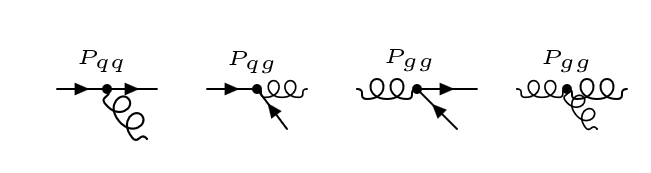
\includegraphics[width=0.85\textwidth]{images/Intro/spiliting.png}
\end{figure}

\begin{equation}
	\left.\begin{aligned}
\langle\:\hat{P_{qq}}\rangle &= C_F[\frac{1+z^2}{1-z}-\varepsilon(1-z)]\\
\langle\:\hat{P_{gq}}\rangle &= T_R[1-\frac{2z(1-z)}{1-\varepsilon}]\\
\langle\:\hat{P_{qg}}\rangle &= C_F[\frac{1+(1-z)^2}{z}-\varepsilon z]\\
\langle\:\hat{P_{gg}}\rangle &= 2C_A[\frac{z}{1-z}+\frac{1-z}{z}+z(1-z)]
\end{aligned}
	\right\}
	\quad \text{splitting functions}
\end{equation}
\newpage
\section{splitting/subtraction method}

\section{Catani-Seymour Formalism}